\documentclass[11pt]{report}

% Paquetes y configuraciones adicionales
\usepackage{amsmath, amsthm, amssymb} % Paquetes matemáticos
\usepackage[utf8]{inputenc} % Codificación .tex
\usepackage[T1]{fontenc} % Codificación .pdf
\usepackage{graphicx}
\usepackage[export]{adjustbox}
\usepackage{caption}
\usepackage{float}
\usepackage{titlesec}
\usepackage{geometry}
\usepackage[hidelinks]{hyperref}
\usepackage{titling}
\usepackage{titlesec}
\usepackage{parskip}
\usepackage{wasysym}
\usepackage{tikzsymbols}
\usepackage{fancyvrb}
\usepackage{xurl}
\usepackage{hyperref}
\usepackage{subcaption}
\usepackage{listings}
\usepackage{xcolor}
\usepackage[spanish]{babel}


\newcommand{\subtitle}[1]{
  \posttitle{
    \par\end{center}
    \begin{center}\large#1\end{center}
    \vskip0.5em}
}

% Configura los márgenes
\geometry{
  left=2cm,   % Ajusta este valor al margen izquierdo deseado
  right=2cm,  % Ajusta este valor al margen derecho deseado
  top=3cm,
  bottom=3cm,
}

% Configuración de los títulos de las secciones
\titlespacing{\section}{0pt}{\parskip}{\parskip}
\titlespacing{\subsection}{0pt}{\parskip}{\parskip}
\titlespacing{\subsubsection}{0pt}{\parskip}{\parskip}

% Redefinir el formato de los capítulos y añadir un punto después del número
\makeatletter
\renewcommand{\@makechapterhead}[1]{%
  \vspace*{0\p@} % Ajusta este valor para el espaciado deseado antes del título del capítulo
  {\parindent \z@ \raggedright \normalfont
    \ifnum \c@secnumdepth >\m@ne
        \huge\bfseries \thechapter.\ % Añade un punto después del número
    \fi
    \interlinepenalty\@M
    #1\par\nobreak
    \vspace{10pt} % Ajusta este valor para el espacio deseado después del título del capítulo
  }}
\makeatother

% Configura para que cada \chapter no comience en una pagina nueva
\makeatletter
\renewcommand\chapter{\@startsection{chapter}{0}{\z@}%
    {-3.5ex \@plus -1ex \@minus -.2ex}%
    {2.3ex \@plus.2ex}%
    {\normalfont\Large\bfseries}}
\makeatother

\definecolor{mygreen}{RGB}{0,128,0}  % Definir el color verde (0,128,0)
\definecolor{myblue}{RGB}{0,0,128}   % Definir el color azul (0,0,128)

\begin{document}

% Portada del informe
\title{Informe de prácticas}
\subtitle{Robótica Computacional}
\author{Cheuk Kelly Ng Pante (alu0101364544@ull.edu.es)}
\date{\today}

\maketitle

\pagestyle{empty} % Desactiva la numeración de página para el índice

% Índice
\tableofcontents

% Nueva página
\newpage

\pagestyle{plain} % Vuelve a activar la numeración de página
\setcounter{page}{1} % Reinicia el contador de página a 1

% Secciones del informe
% Capitulo 1
\chapter{Cinematica Directa}
La cinemática directa es una rama de la robótica y la mecánica que se ocupa de la relación entre los movimientos
de los eslabones de un robot y las variables que los controlan. En otras palabras, la cinemática directa es el
problema de encontrar la posición y orientación del extremo del robot, dado el conjunto de parámetros que
definen las posiciones y orientaciones de todos los eslabones.

Para explicar la cinemática directa, se utilizará el sistema de coordenadas de Denavit-Hartenberg (DH). El sistema
de coordenadas de Denavit-Hartenberg es un sistema de coordenadas utilizado para modelar cinemática directa e
inversa de robots articulados. El sistema de coordenadas de Denavit-Hartenberg se basa en cuatro parámetros
asociados a cada articulación. Estos parámetros son:
\begin{itemize}
  \item $d_i$: Distancia entre los ejes $z_{i-1}$ y $z_i$ a lo largo del eje $x_i$.
  \item $\theta_i$: Ángulo entre los ejes $z_{i-1}$ y $z_i$ alrededor del eje $x_i$.
  \item $a_i$: Distancia entre los ejes $x_{i-1}$ y $x_i$ a lo largo del eje $z_{i-1}$.
  \item $\alpha_i$: Ángulo entre los ejes $x_{i-1}$ y $x_i$ alrededor del eje $z_{i-1}$.
\end{itemize}

Los parámetros DH se pueden calcular segun la tabla siguiente:
\begin{table}[H]
  \centering
  \begin{tabular}{|c|c|c|c|}
    \hline
    \textbf{}           & \textbf{A}                 & \textbf{B}                 & \textbf{C}         \\ \hline
    \textbf{$d_i$}      & \texttt{$O_{i-1}$}         & \texttt{$Z_{i-1}\cap X_i$} & \texttt{$Z_{i-1}$} \\ \hline
    \textbf{$\theta_i$} & \texttt{$X_{i-1}$}         & \texttt{$X_{i}$}           & \texttt{$Z_{i-1}$} \\ \hline
    \textbf{$a_i$}      & \texttt{$Z_{i-1}\cap X_i$} & \texttt{$O_{i}$}           & \texttt{$X_{i}$}   \\ \hline
    \textbf{$\alpha_i$} & \texttt{$Z_{i-1}$}         & \texttt{$Z_{i}$}           & \texttt{$X_{i}$}   \\ \hline
  \end{tabular}
  \caption{Parámetros DH}
\end{table}

Para la explicación de la cinemática directa, se utilizará el manipulador 3:
\begin{figure}[H]
  \centering
  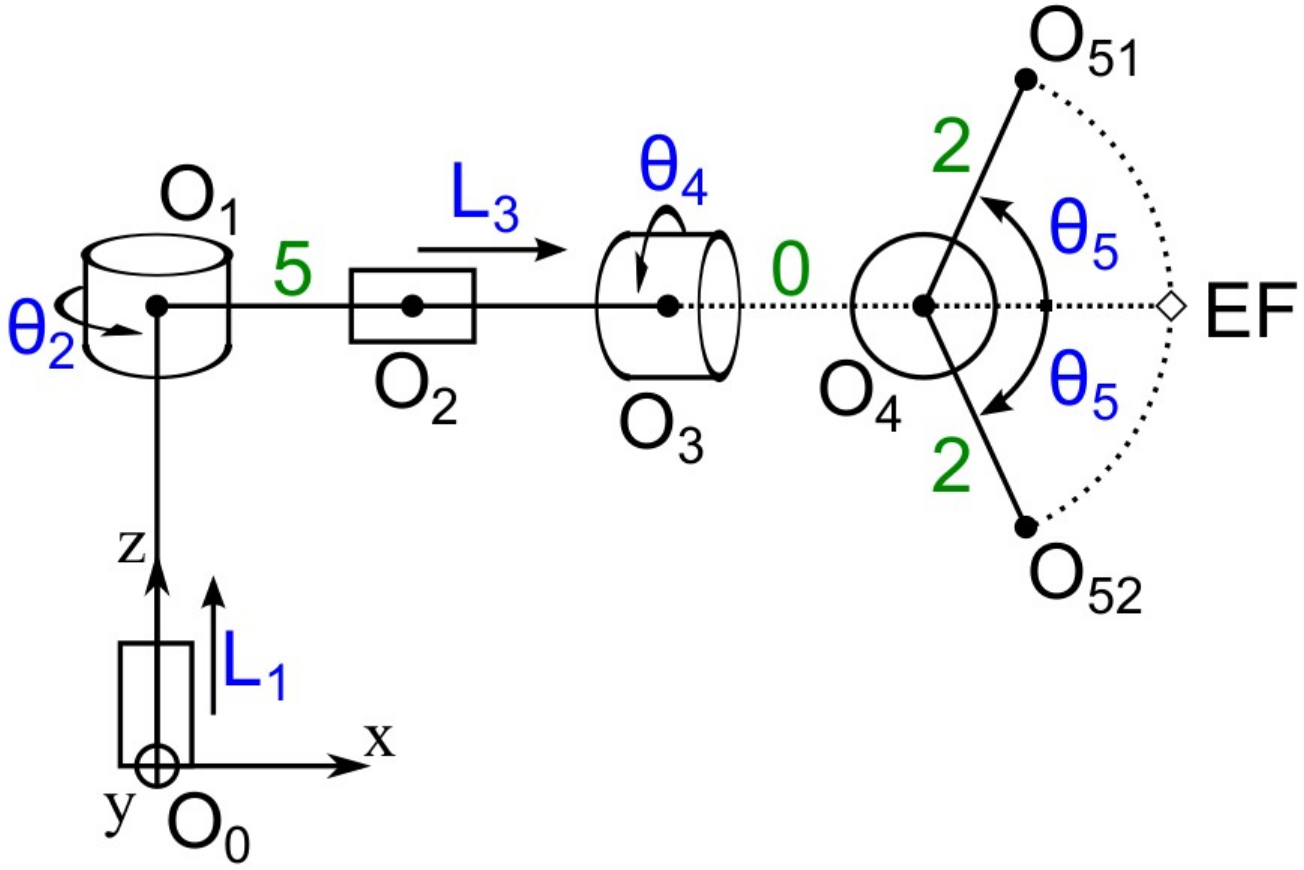
\includegraphics[scale=0.24]{img/manipulador.png}
  \caption{Manipulador ejemplo}
\end{figure}
Para calcular la cinemática directa, primero vamos a calcular los parámetros DH:
\begin{figure}[H]
  \centering
  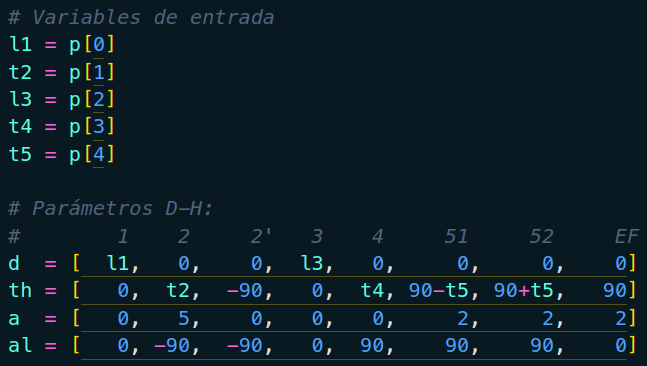
\includegraphics[scale=0.4]{img/parametros_dh.png}
  \caption{Parámetros DH del manipulador 3}
\end{figure}

Como se puede observar en la figura 1.2, antes de calcular los parámetros DH, se ha
asignado unas variables de entrada, estas corresponden a los ángulos de las articulaciones del manipulador
y estas son los valores que se introducen al ejecutar el programa. Por ejemplo, si lo ejecutamos de la siguiente
manera:
\begin{verbatim}
$ python3 ./cinematica_directa 5 0 5 90 45
\end{verbatim}

el resultado de la cinemática directa sería la siguiente:
\begin{figure}[H]
  \centering
  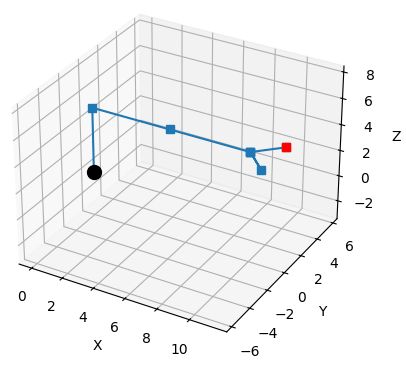
\includegraphics[scale=0.7]{img/cinematica_directa.png}
  \caption{Cinemática directa del manipulador 3}
\end{figure}

\newpage

Después, se calculado la matriz de transformación de cada articulación para este manipulador:
\begin{figure}[H]
  \centering
  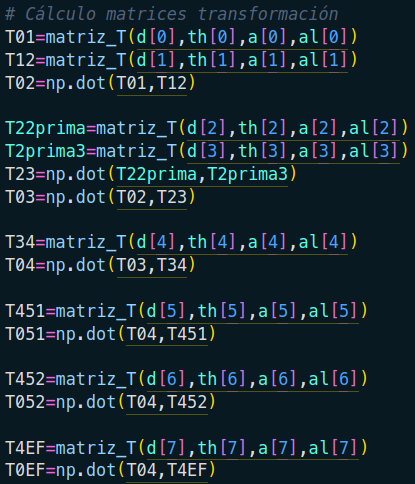
\includegraphics[scale=0.5]{img/matriz_transformacion.png}
  \caption{Matriz de transformación del manipulador 3}
\end{figure}

Luego, la transformación de cada articulación, especificando los datos de la tabla de Denavit Hartenberg especificadas en la figura 1.2:
\begin{figure}[H]
  \centering
  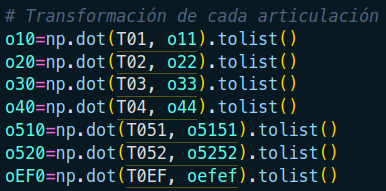
\includegraphics[scale=0.5]{img/transformacion_articulacion.png}
  \caption{Transformación de cada articulación del manipulador 3}
\end{figure}

Y por último, el resultado de la cinemática directa del manipulador 3:
\begin{figure}[H]
  \centering
  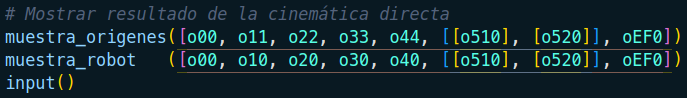
\includegraphics[scale=0.5]{img/resultado_cd.png}
  \caption{Cinemática directa del manipulador 3}
\end{figure}

\newpage

\chapter{Cinematica Inversa}
La cinemática inversa es una rama de la robótica y la mecánica que se ocupa de la relación entre los movimientos
de los eslabones de un robot y las variables que los controlan. En otras palabras, la cinemática inversa es el
problema de encontrar el conjunto de parámetros que definen las posiciones y orientaciones de todos los eslabones,
dado la posición y orientación del extremo del robot.

La cinemática inversa puede ser un problema complejo debido a la presencia de restricciones y limitaciones física
del robot, como por ejemplo, limites de movimientos de las articulaciones, colisiones o singularidades.

En la práctica de la cinemática inversa, se ha de calcular la distancia que debe extenderse una articulación prismática
situada en el punto $O_i$, de tal forma que el punto final del robot $O_n$ se acerque tanto como sea posible a la posición
objetivo R.

El acercamiento solo puede hacerse en la dirección de extensión $L_i$, que se puede calcular como un angulo de $w$ que define
la rotación respecto al eje x absoluto. El angulo $w$ se puede calcular como:
\begin{equation*}
  \color{blue}\omega\color{black} = \sum_{j = 0}^{\color{blue}i\color{black}} \theta_j
\end{equation*}

Usando el producto escalar se puede proyectar el vector que $O_n$ hasta $R$ sobre la dirección de extensión de la articulacion
obteniendo así la distancia $d$:
\begin{equation*}
  \color{green} \mathbf{d} \color{black} =
  \begin{bmatrix}
    \cos(\color{blue}\omega\color{black}) \\
    \sin(\color{blue}\omega\color{black})
  \end{bmatrix}
  \cdot (\color{red}R\color{black}- \color{red}\text{ON}\color{black})
\end{equation*}


\end{document}